
%(BEGIN_QUESTION)
% Copyright 2010, Tony R. Kuphaldt, released under the Creative Commons Attribution License (v 1.0)
% This means you may do almost anything with this work of mine, so long as you give me proper credit

When two gears mesh together, their rotational speeds and torques are both related to the ratio of diameters (also the same as the ratio of gear teeth, since the teeth on each gear must be identically sized in order to properly mesh).  For example, if one gear having 35 teeth meshes with a second gear of equal diameter (also having 35 teeth), the gear ratio will be 1:1, which means they will rotate at exactly the same speed and with exactly the same amount of torque.

\vskip 10pt

Suppose two gears mesh together to form a speed reduction mechanism, with the following diameters:

$$\includegraphics[width=15.5cm]{i01405x01.eps}$$

Based on this diagram of the two gears, answer these questions:

\begin{itemize}
\item{} Calculate the {\it gear ratio} of this gear set.
\vskip 10pt
\item{} If the first gear's shaft exerts a torque of 600 lb-ft on the gear (the ``input'' torque), how much torque will be exerted on the second gear's shaft (the ``output'' torque)?
\vskip 10pt
\item{} If the input gear spins at 200 RPM, how fast does the output gear spin?
\vskip 10pt
\item{} If the small gear has 24 teeth, how many teeth will the large gear have?
\end{itemize}

\vskip 20pt \vbox{\hrule \hbox{\strut \vrule{} {\bf Suggestions for Socratic discussion} \vrule} \hrule}

\begin{itemize}
\item{} Use the torque formula $\vec \tau = \vec r \times \vec F$ (torque being the product of radius and linear force) to solve for the torque ratio $\left( \tau_1 \over \tau_2 \right)$ knowing the diameter (or radius) ratio of two meshing gears.
\item{} Use the speed formula $v = r\omega$ (rim velocity being the product of radius and rotational speed) to solve for the rotational speed ratio $\left( \omega_1 \over \omega_2 \right)$ knowing the diameter (or radius) ratio of two meshing gears.
\end{itemize}

\underbar{file i01405}
%(END_QUESTION)





%(BEGIN_ANSWER)

\noindent
{\bf Partial answer:}

\begin{itemize}
\item{} If the first gear's shaft exerts a torque of 600 lb-ft on the gear (the ``input'' torque), how much torque will be exerted on the second gear's shaft (the ``output'' torque)?  {\it $\tau_{output}$ = 3,400 lb-ft}
\vskip 10pt
\item{} If the small gear has 24 teeth, how many teeth will the large gear have?  {\it 136 teeth}
\end{itemize}
 
%(END_ANSWER)





%(BEGIN_NOTES)

\begin{itemize}
\item{} Calculate the {\it gear ratio} of this gear set.  {\it Gear ratio = 17/3 = 5.667:1}
\vskip 10pt
\item{} If the first gear's shaft exerts a torque of 600 lb-ft on the gear (the ``input'' torque), how much torque will be exerted on the second gear's shaft (the ``output'' torque)?  {\it $\tau_{output}$ = (600 lb-ft)(17/3) = 3,400 lb-ft}
\vskip 10pt
\item{} If the input gear spins at 200 RPM, how fast does the output gear spin?  {\it $S_{output}$ = (200 RPM)(3/17) = 35.29 RPM}
\vskip 10pt
\item{} If the small gear has 24 teeth, how many teeth will the large gear have?  {\it (24)(17/3) = 136 teeth}
\end{itemize}

%INDEX% Physics, torque: definition
%INDEX% Physics, torque: calculation problem

%(END_NOTES)


